\documentclass[11pt, a4paper]{article}
\usepackage{pdfpages}
\usepackage{parallel}
\usepackage[T2A]{fontenc}
\usepackage{ucs}
\usepackage[utf8x]{inputenc}
\usepackage[polish,english,russian]{babel}
\usepackage{hyperref}
\usepackage{rotating}
\usepackage[inner=2cm,top=1.8cm,outer=2cm,bottom=2.3cm,nohead]{geometry}
\usepackage{listings}
\usepackage{graphicx}
\usepackage{wrapfig}
\usepackage{longtable}
\usepackage{indentfirst}
\usepackage{array}
\usepackage{tikzsymbols}
\usepackage{soul}
\usepackage[ruled,vlined]{algorithm2e}
%\counterwithout{figure}{section} 

\usepackage{url}
\makeatletter
\g@addto@macro{\UrlBreaks}{\UrlOrds}
\makeatother

\newcolumntype{P}[1]{>{\raggedright\arraybackslash}p{#1}}
\frenchspacing
\usepackage{fixltx2e} %text sub- and superscripts
\usepackage{icomma} % коскі ў матэматычным рэжыме
\PreloadUnicodePage{4}

\newcommand{\longpage}{\enlargethispage{\baselineskip}}
\newcommand{\shortpage}{\enlargethispage{-\baselineskip}}

\def\switchlang#1{\expandafter\csname switchlang#1\endcsname}
\def\switchlangbe{
\let\saverefname=\refname%
\def\refname{Літаратура}%
\def\figurename{Іл.}%
}
\def\switchlangen{
\let\saverefname=\refname%
\def\refname{References}%
\def\figurename{Fig.}%
}
\def\switchlangru{
\let\saverefname=\refname%
\let\savefigurename=\figurename%
\def\refname{Литература}%
\def\figurename{Рис.}%
}

\hyphenation{admi-ni-stra-tive}
\hyphenation{ex-pe-ri-ence}
\hyphenation{fle-xi-bi-li-ty}
\hyphenation{Py-thon}
\hyphenation{ma-the-ma-ti-cal}
\hyphenation{re-ported}
\hyphenation{imp-le-menta-tions}
\hyphenation{pro-vides}
\hyphenation{en-gi-neering}
\hyphenation{com-pa-ti-bi-li-ty}
\hyphenation{im-pos-sible}
\hyphenation{desk-top}
\hyphenation{elec-tro-nic}
\hyphenation{com-pa-ny}
\hyphenation{de-ve-lop-ment}
\hyphenation{de-ve-loping}
\hyphenation{de-ve-lop}
\hyphenation{da-ta-ba-se}
\hyphenation{plat-forms}
\hyphenation{or-ga-ni-za-tion}
\hyphenation{pro-gramming}
\hyphenation{in-stru-ments}
\hyphenation{Li-nux}
\hyphenation{sour-ce}
\hyphenation{en-vi-ron-ment}
\hyphenation{Te-le-pathy}
\hyphenation{Li-nux-ov-ka}
\hyphenation{Open-BSD}
\hyphenation{Free-BSD}
\hyphenation{men-ti-on-ed}
\hyphenation{app-li-ca-tion}

\def\progref!#1!{\texttt{#1}}
\renewcommand{\arraystretch}{2} %Іначай формулы ў матрыцы зліпаюцца з лініямі
\usepackage{array}

\def\interview #1 (#2), #3, #4, #5\par{

\section[#1, #3, #4]{#1 -- #3, #4}
\def\qname{LVEE}
\def\aname{#1}
\def\q ##1\par{{\noindent \bf \qname: ##1 }\par}
\def\a{{\noindent \bf \aname: } \def\qname{L}\def\aname{#2}}
}

\def\interview* #1 (#2), #3, #4, #5\par{

\section*{#1\\{\small\rm #3, #4. #5}}
\ifx\ParallelWhichBox\undefined%
    \addcontentsline{toc}{section}{#1, #3, #4}%
\else%
\ifnum\ParallelWhichBox=0%
    \addcontentsline{toc}{section}{#1, #3, #4}%
\fi\fi%

\def\qname{LVEE}
\def\aname{#1}
\def\q ##1\par{{\noindent \bf \qname: ##1 }\par}
\def\a{{\noindent \bf \aname: } \def\qname{L}\def\aname{#2}}
}

\newcommand{\interviewfooter}[1]{
\vskip 1em
\noindent \textit{#1}
}

\switchlang{en}
\begin{document}

\title{1993 "--- Evergreen Diamond XL trackball}
\date{}
\maketitle
\selectlanguage{english}
The Diamond XL trackball was produced by the Evergreen Systems International company in California, founded in 1980 and specialized in high-quality trackballs for industrial and military applications.

Diamond trackballs have been positioned as a mouse replacement in computer systems where fast and precise pointing is required (CAD/CAM, graphics, workstations, kiosks, etc.) and in industrial and military systems where a mouse is not suitable due to lack of space, harsh environment or other factors.

The first mentions of this model in promotional materials date back to 1993 \cite{nasa}.

\begin{figure}[h]
    \centering
    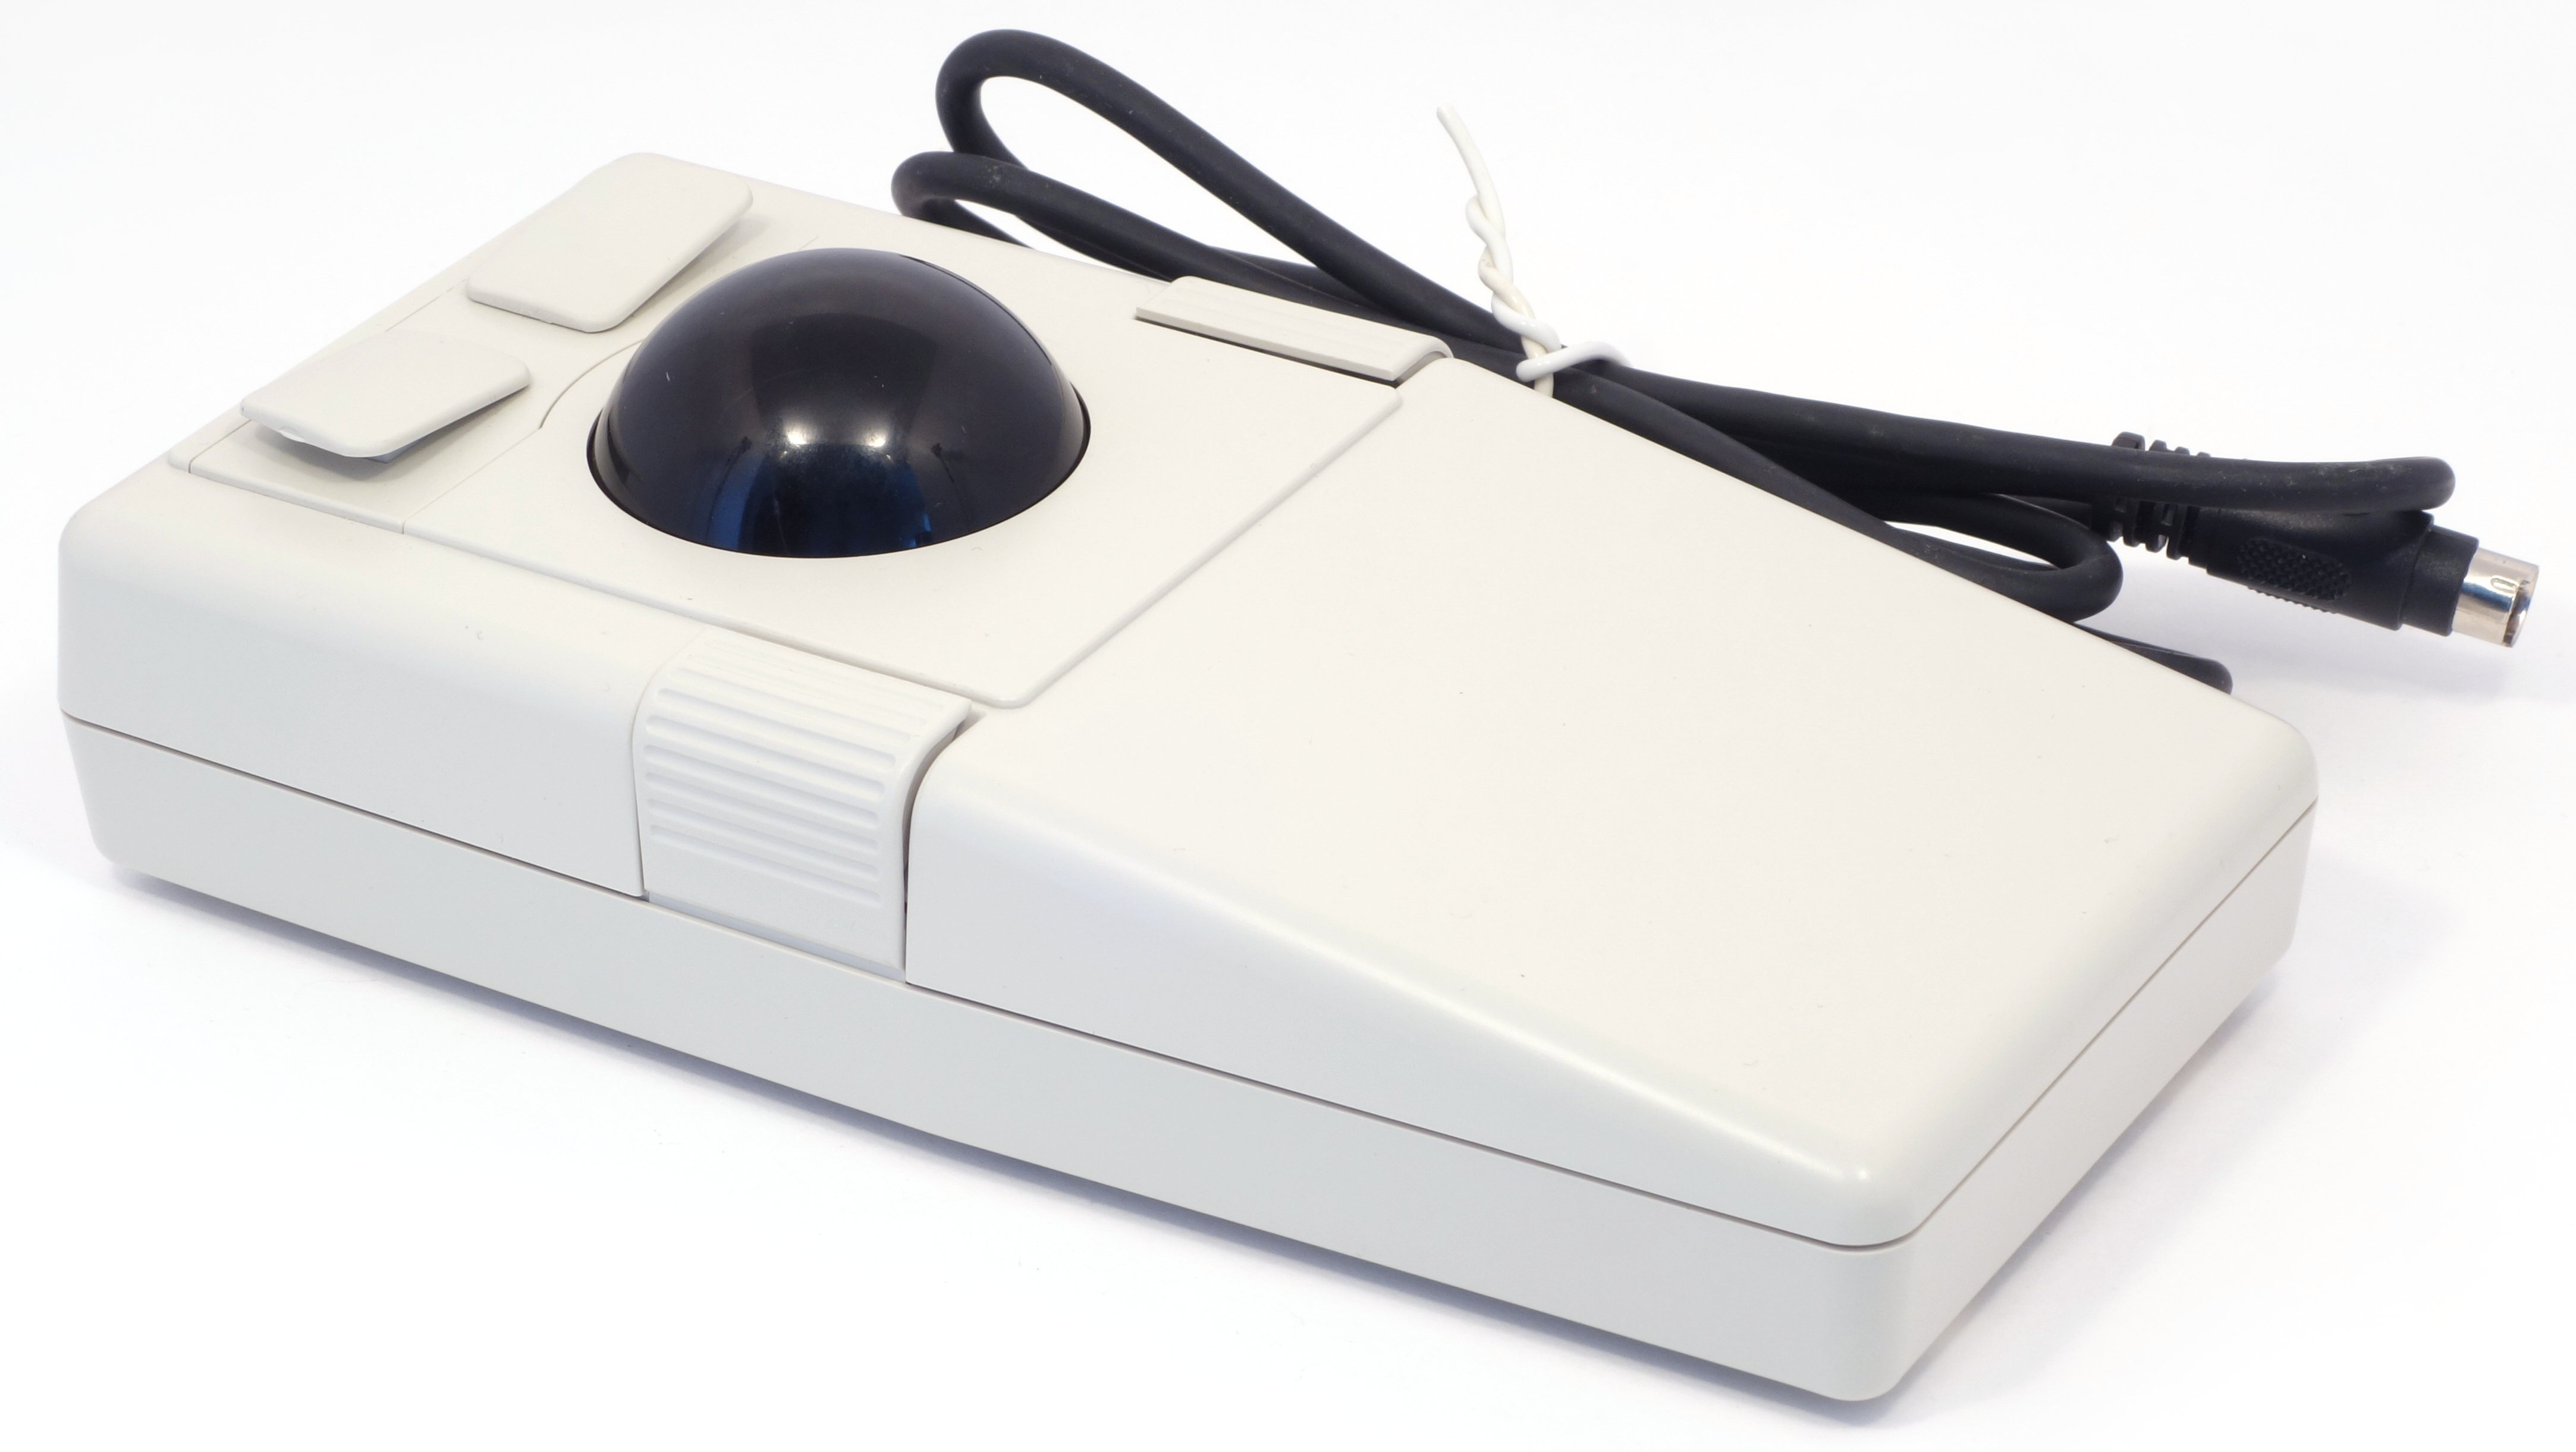
\includegraphics[scale=0.33]{1993_evergreen_diamond_xl_trackball/pic_30.jpg}
    \caption{Diamond XL trackball}
    \label{fig:DiamondXL}
\end{figure}

Figure \ref{fig:DiamondXLTopBottom} shows top and bottom sides of the trackball.
There is no any labels on the top of the case; it has a smooth matte surface and ribbed side keys for easier tactile identification. On the bottom of the case there are rubber feet that provide a secure fit on the table surface, as well as labels specifying the manufacturer and model.

\begin{figure}[h]
    \centering
    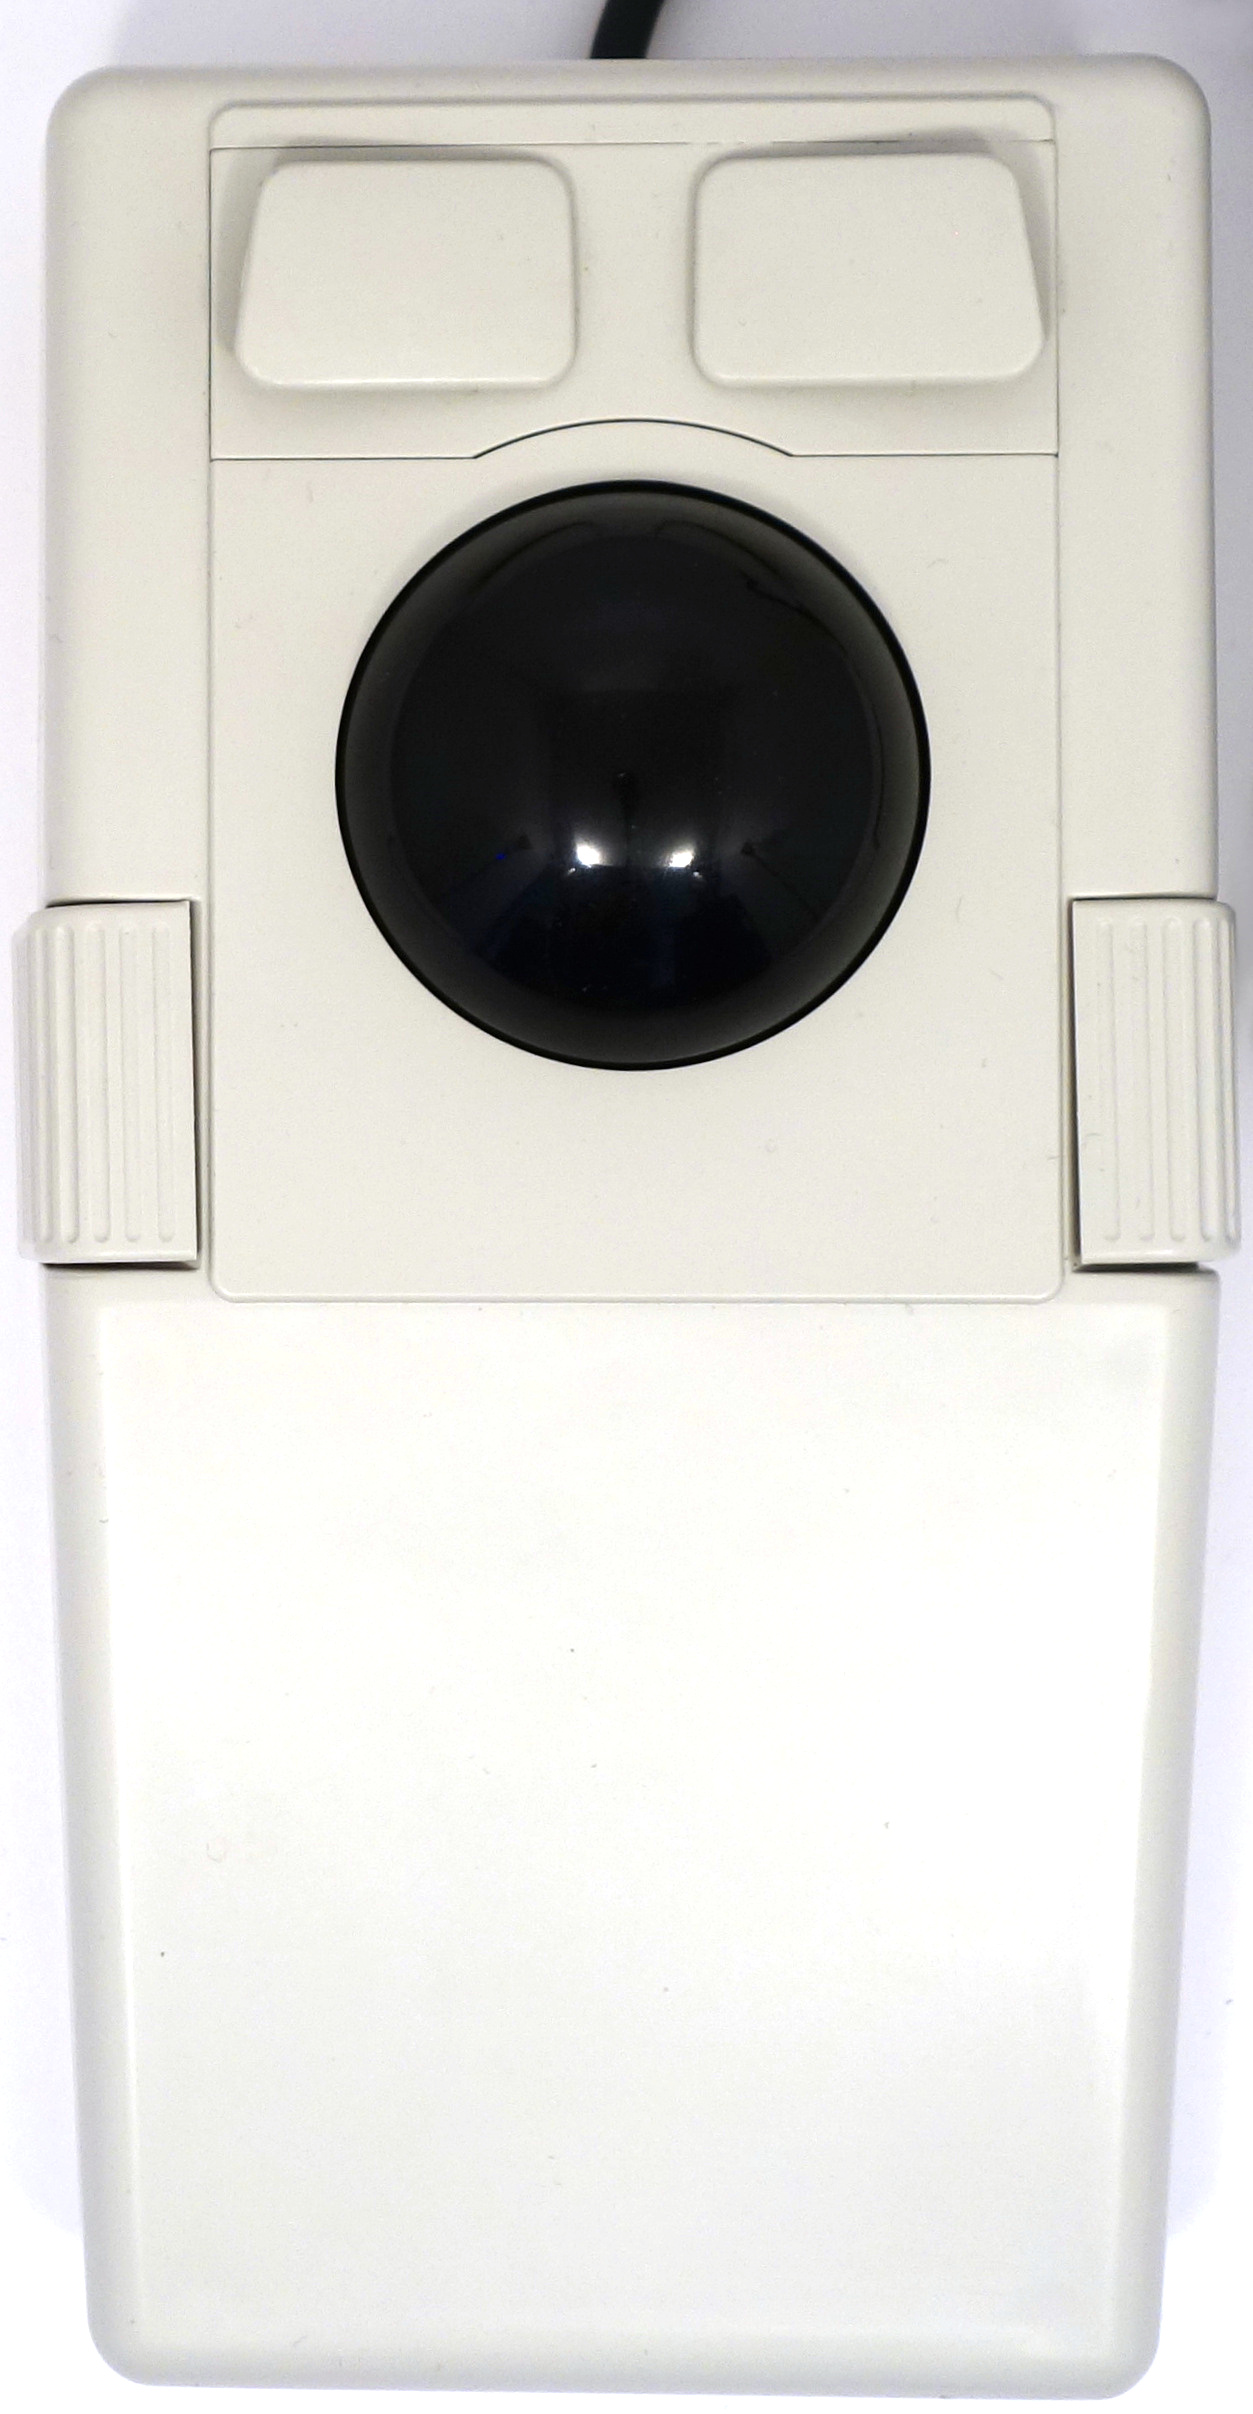
\includegraphics[scale=0.35]{1993_evergreen_diamond_xl_trackball/top_30.jpg}
    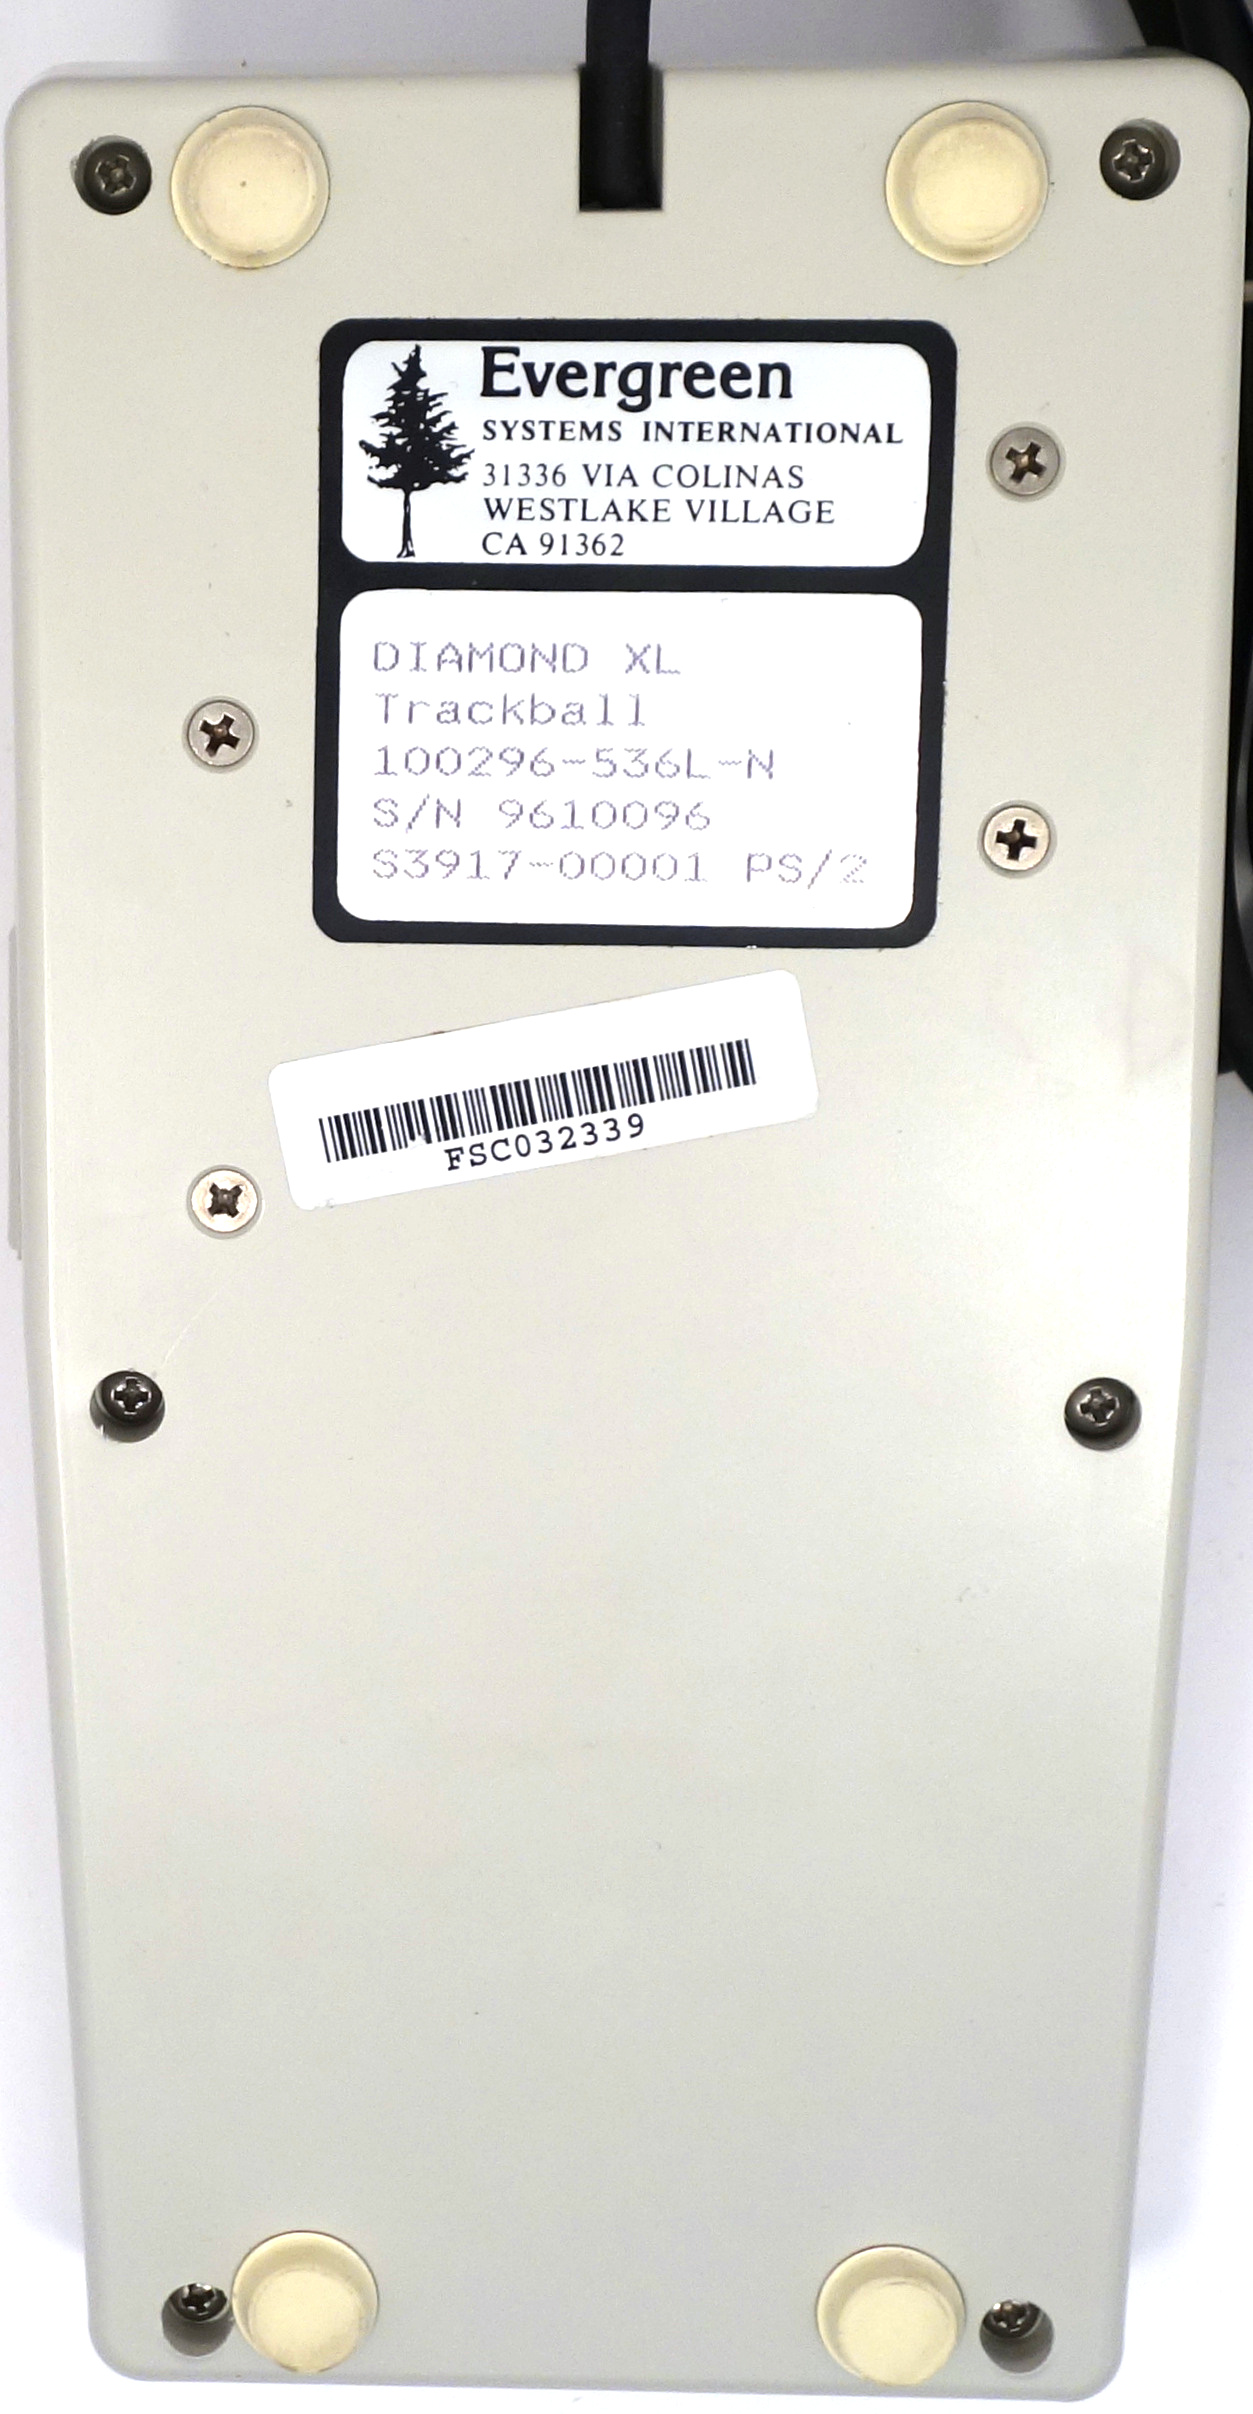
\includegraphics[scale=0.35]{1993_evergreen_diamond_xl_trackball/bottom_30.jpg}
    \caption{Diamond XL trackball top and bottom views}
     \label{fig:DiamondXLTopBottom}
\end{figure}

This device is quite large (fig. \ref{fig:DiamondXLSize}). The ball has diameter of 51 mm (2 inches).

\begin{figure}[h]
    \centering
    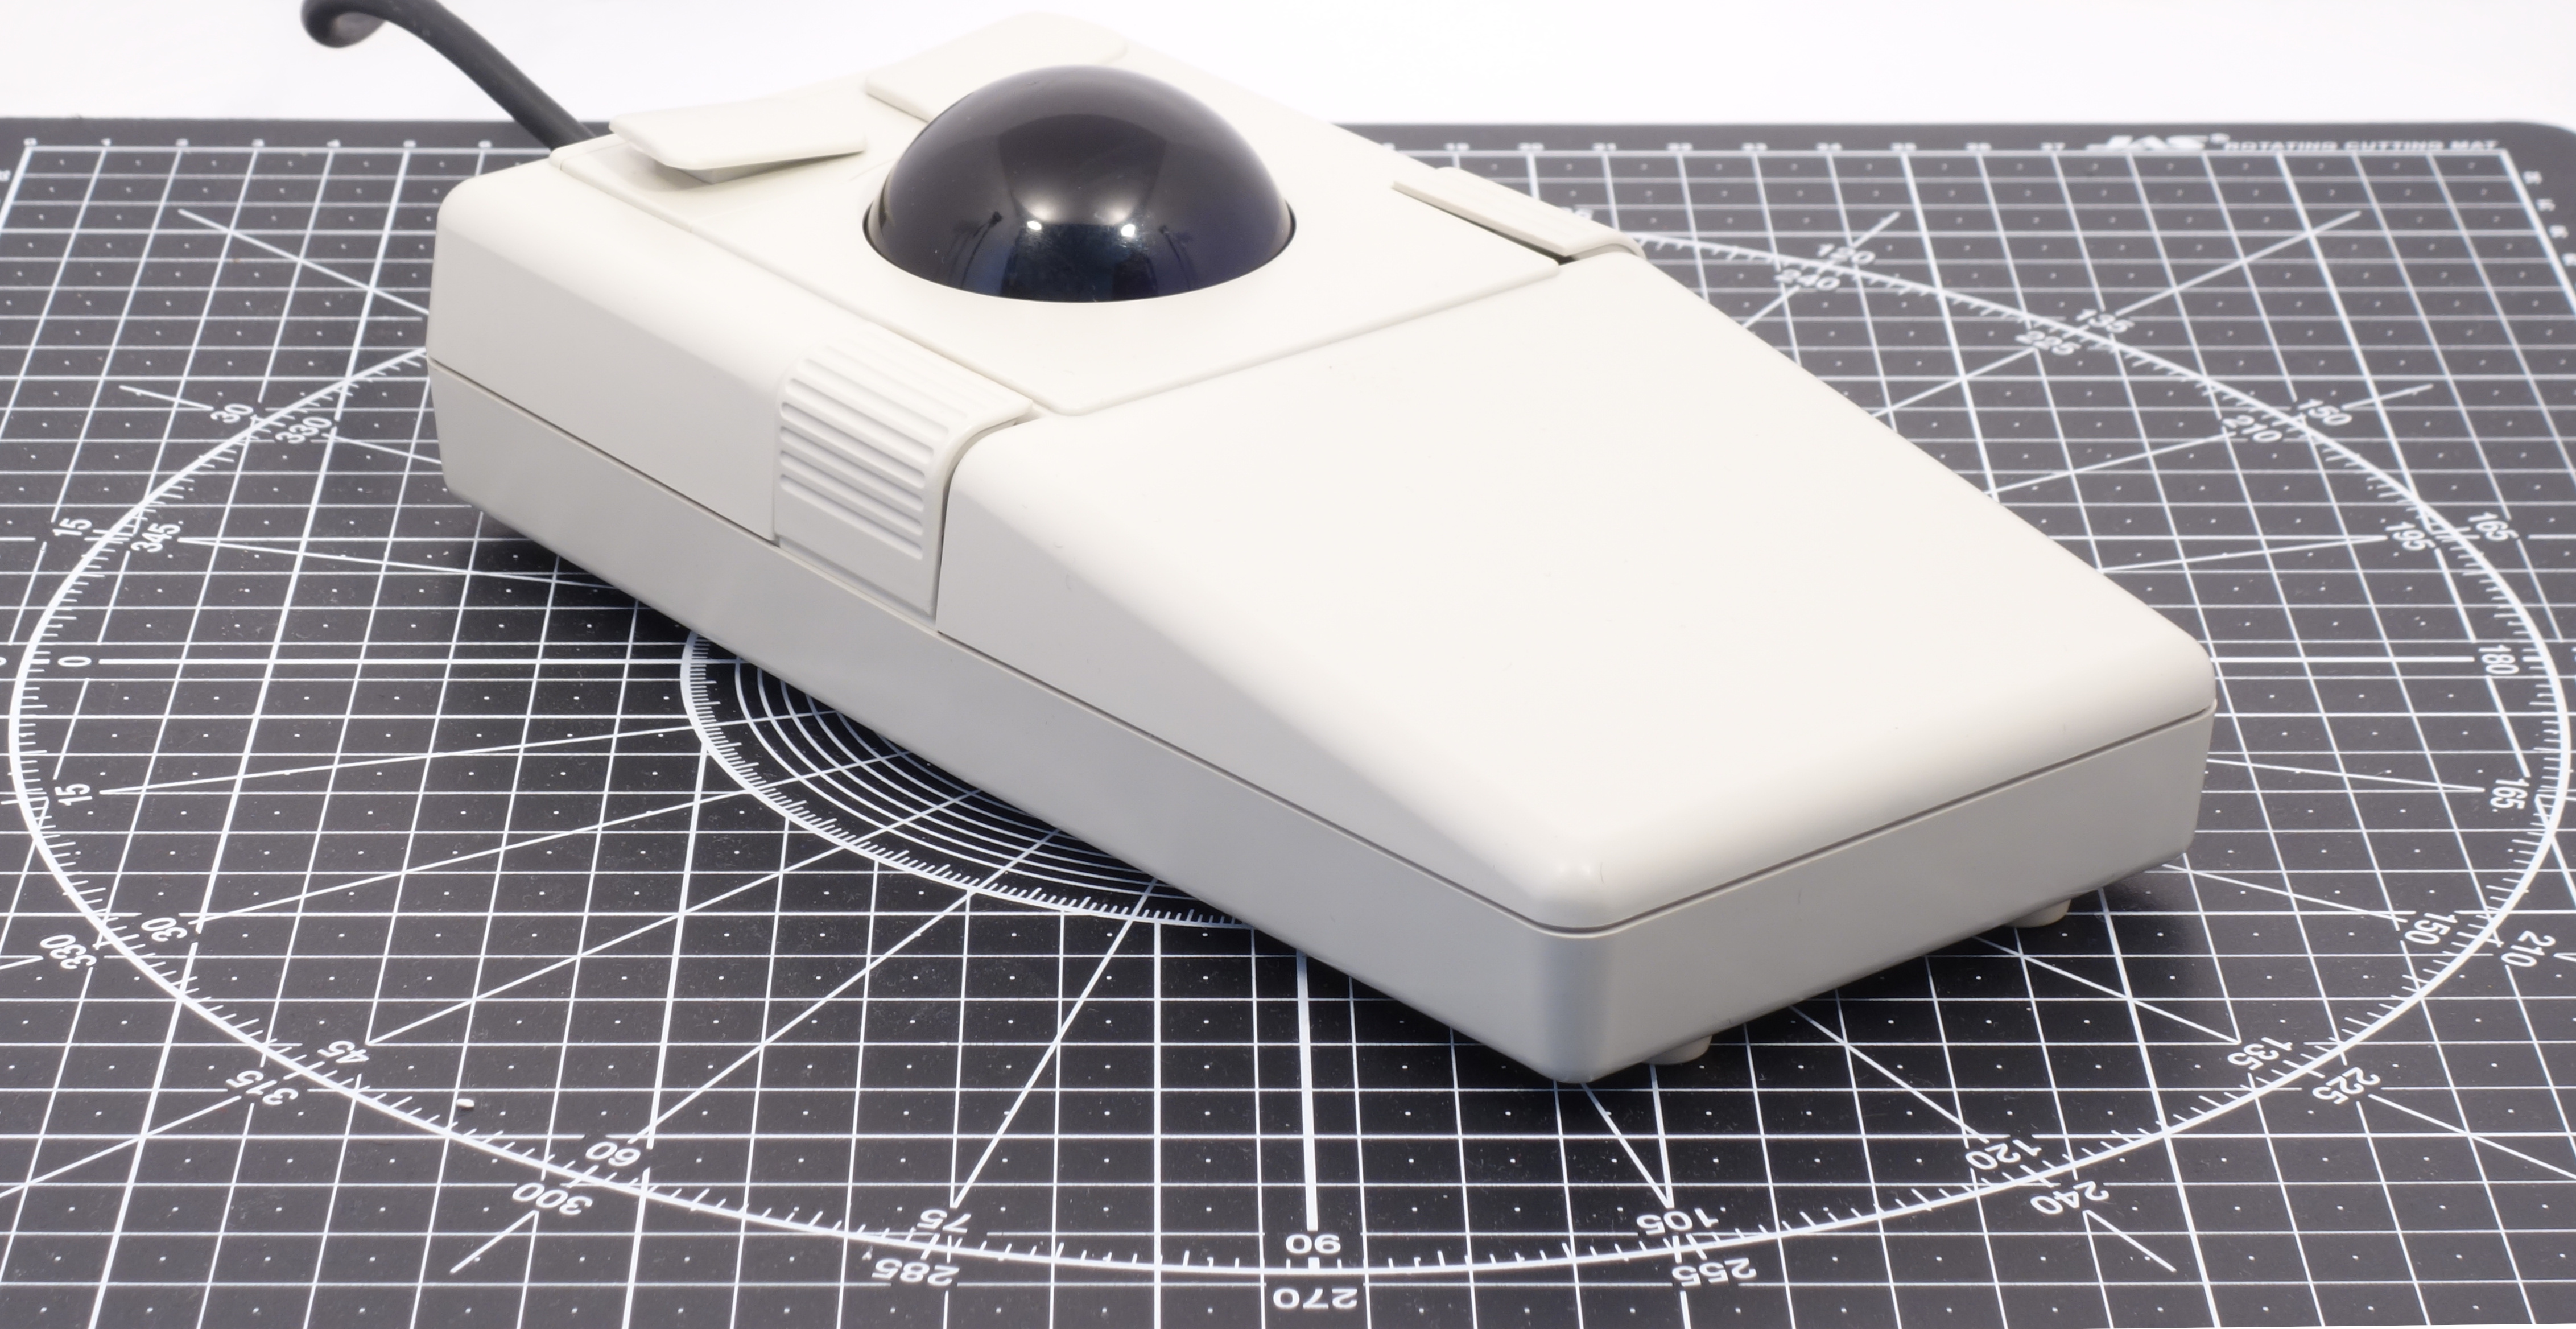
\includegraphics[scale=0.35]{1993_evergreen_diamond_xl_trackball/size.jpg}
    \caption{Diamond XL trackball on a graduated pad with a grid step of 1~cm}
    \label{fig:DiamondXLSize}
\end{figure}

The trackball is symmetrical and equally comfortable when used with both right and left hands. The main (left) mouse button is located under the thumb for easy selection and dragging of objects (fig. \ref{fig:DiamondXLHand}), while the other fingers remain free to position the cursor. The role of the middle button is played by a pair of inclined keys located behind the ball (in this version of the trackball they are inclined towards the center, and in the five-button version \cite{evergreen} mentioned on the manufacturer's website, behind the ball there is a block of three such keys rotated 90 degrees and having slope towards the edge of the body). The right button is symmetrical to the left one and is pressed with the little finger. In some modifications, right-hand or left-hand control is selected using configuration switches located in a cutout in the bottom of the case, but in this sample it is implemented at the driver level only.

The trackball was produced with various interfaces, which allowed it to be used with SUN, DEC, Hewlett Packard (HP/HIL bus), IBM, SGI and USB-equipped Macintosh computers. In particular, the DTXL3 trackball with the HP/HIL bus was produced under license from Hewlett Packard, and was positioned as a direct replacement for the HP/HIL mouse, as well as the discontinued Hewlett Packard HP M1309A trackball \cite{dtxl3, hphil}. 
Traces of such orientation can be seen in the design of the Diamond XL case: the side farthest from the user has two technological rectangles designed to install sockets connecting to the HP/HIL bus (fig. \ref{fig:DiamondXLHand}).

\begin{figure}[h]
    \centering
    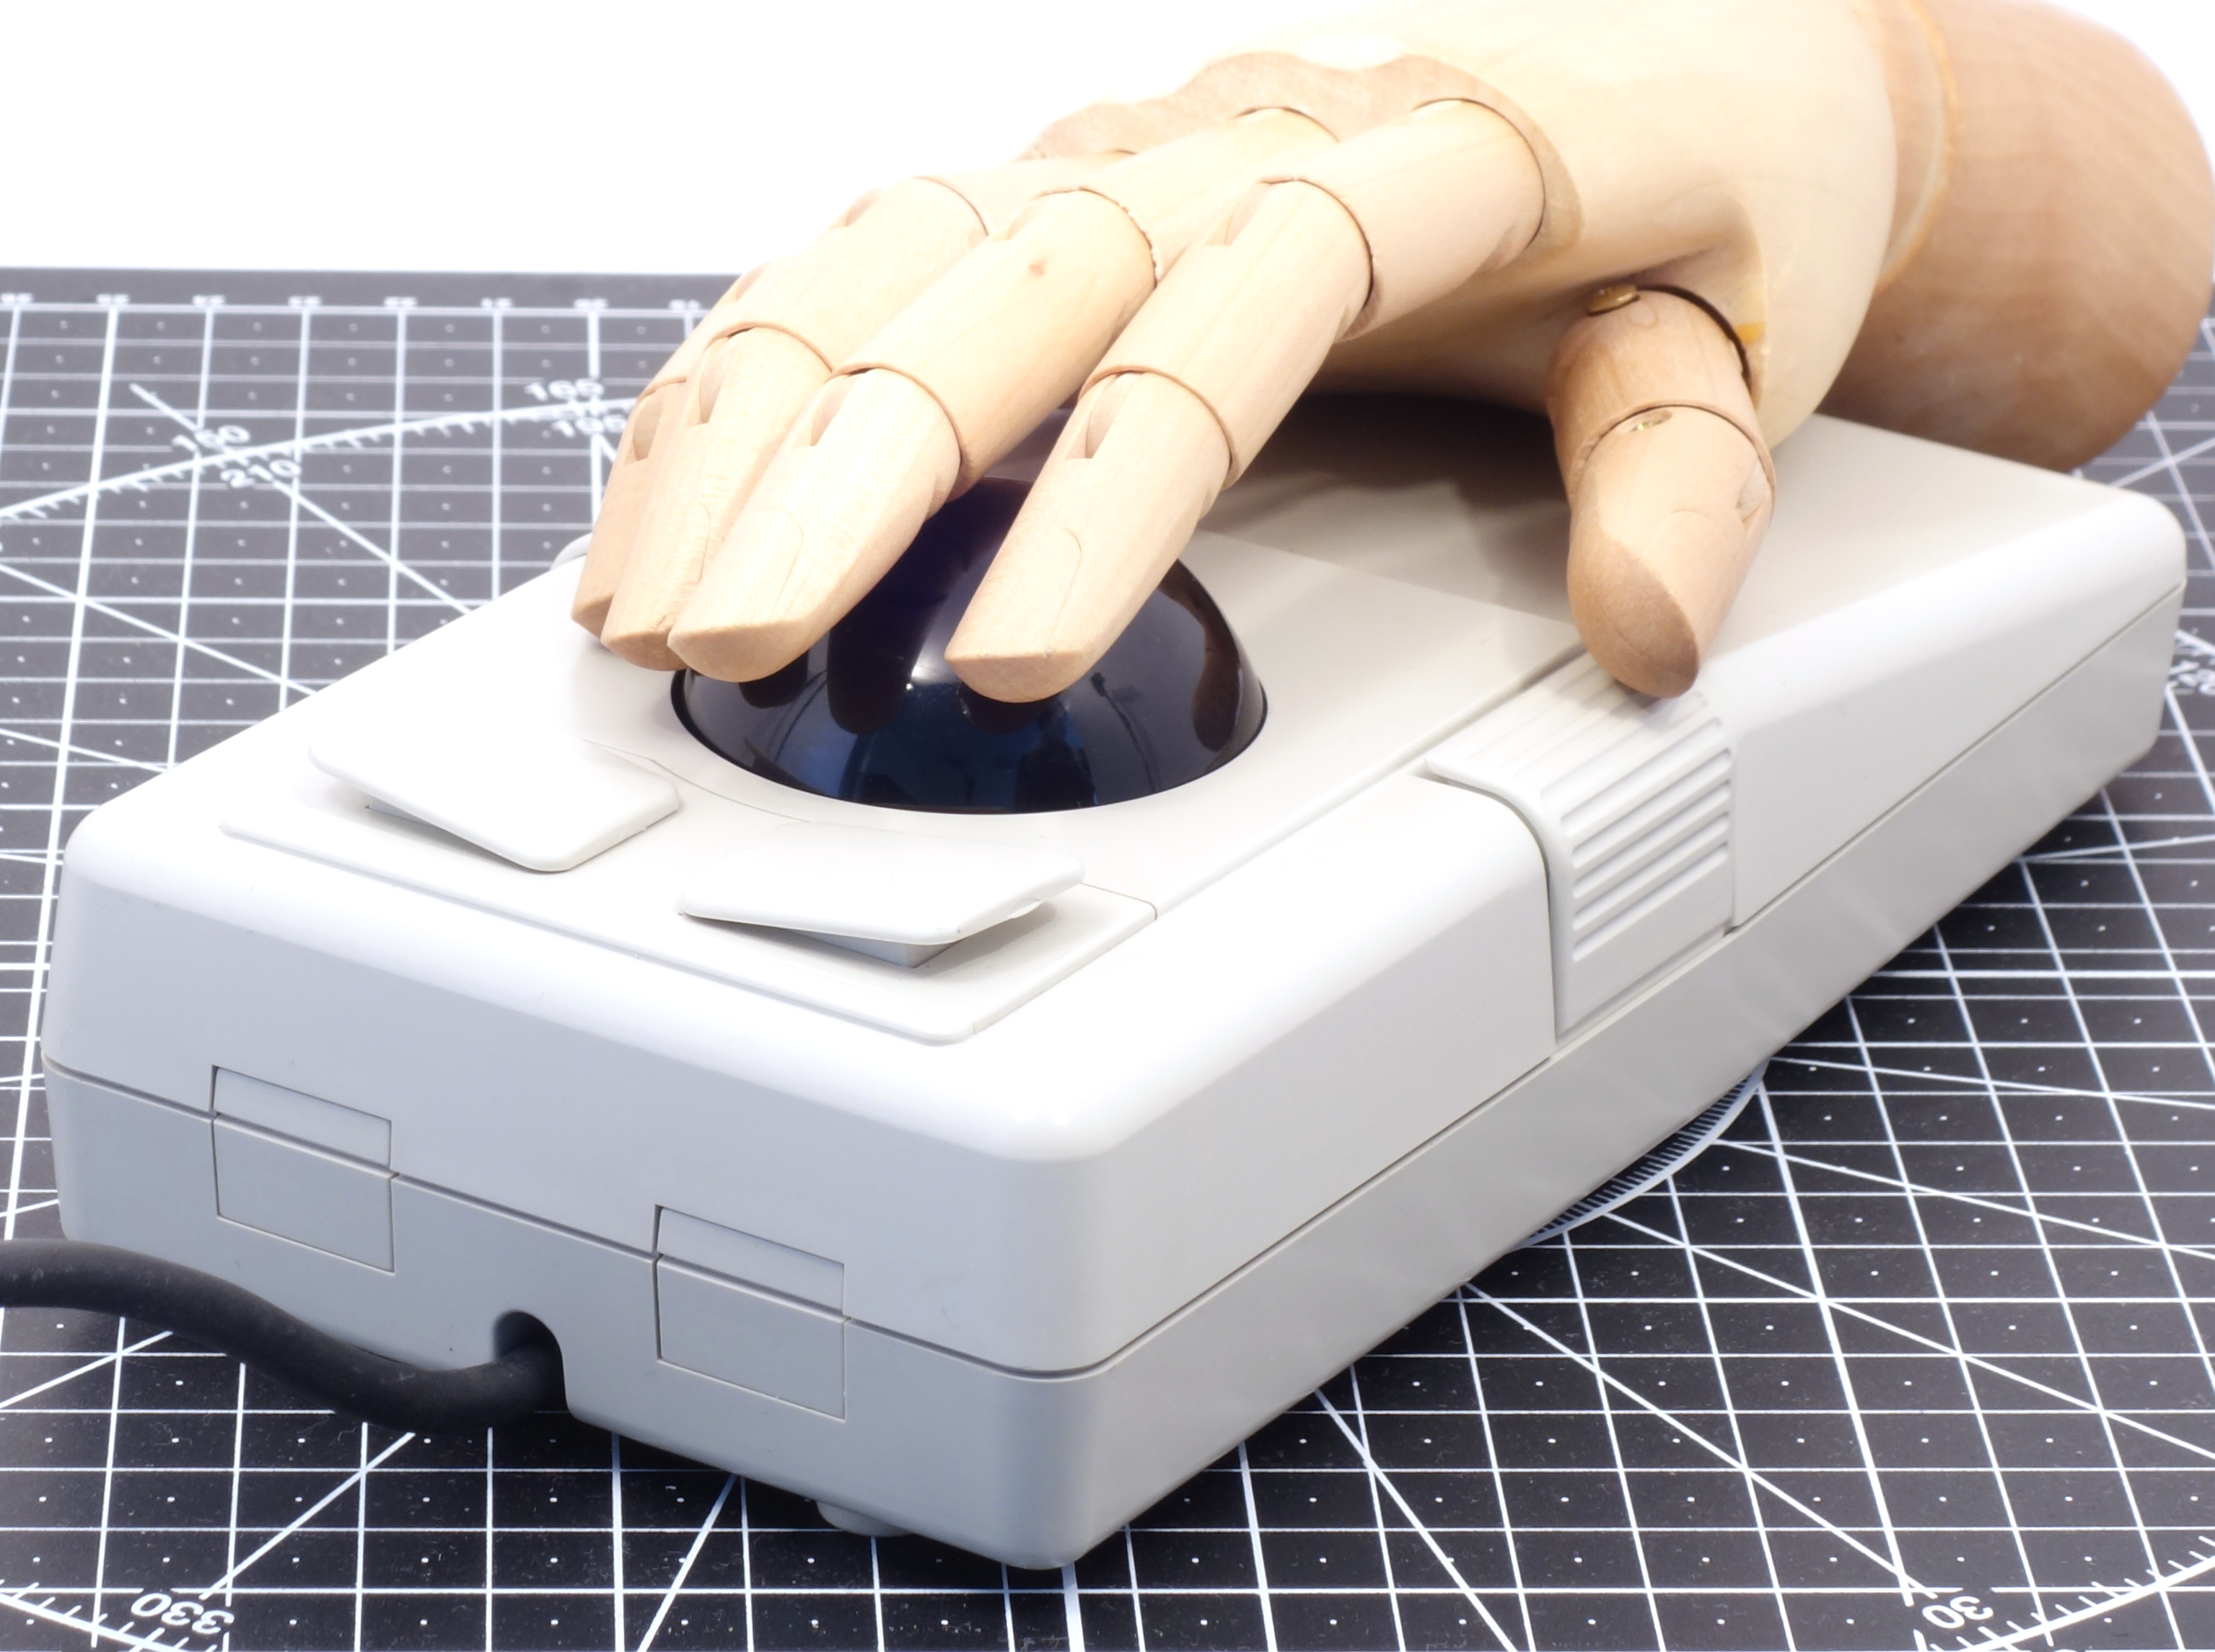
\includegraphics[scale=0.4]{1993_evergreen_diamond_xl_trackball/hand_30.jpg}
    \caption{Diamond XL trackball with a human hand model}
    \label{fig:DiamondXLHand}
\end{figure}

The trackball internals are shown in fig. \ref{fig:DiamondXLInside}. As you can see, this trackball follows the traditional opto-mechanical scheme. It should also be noted that the rollers are implemented using bearings and steel shafts designed to ensure maximum reliability and durability of the device. This is also emphasized in the manufacturer's description, which specially mentions all-metal mechanicals, hard nitrited steel shafts with precision ball bearings and gold-plated spring-contact switches \cite{dtxl3}.

Apparently, it is impossible to get the ball out for cleaning without disassembling the case.


\begin{figure}[h]
    \centering
    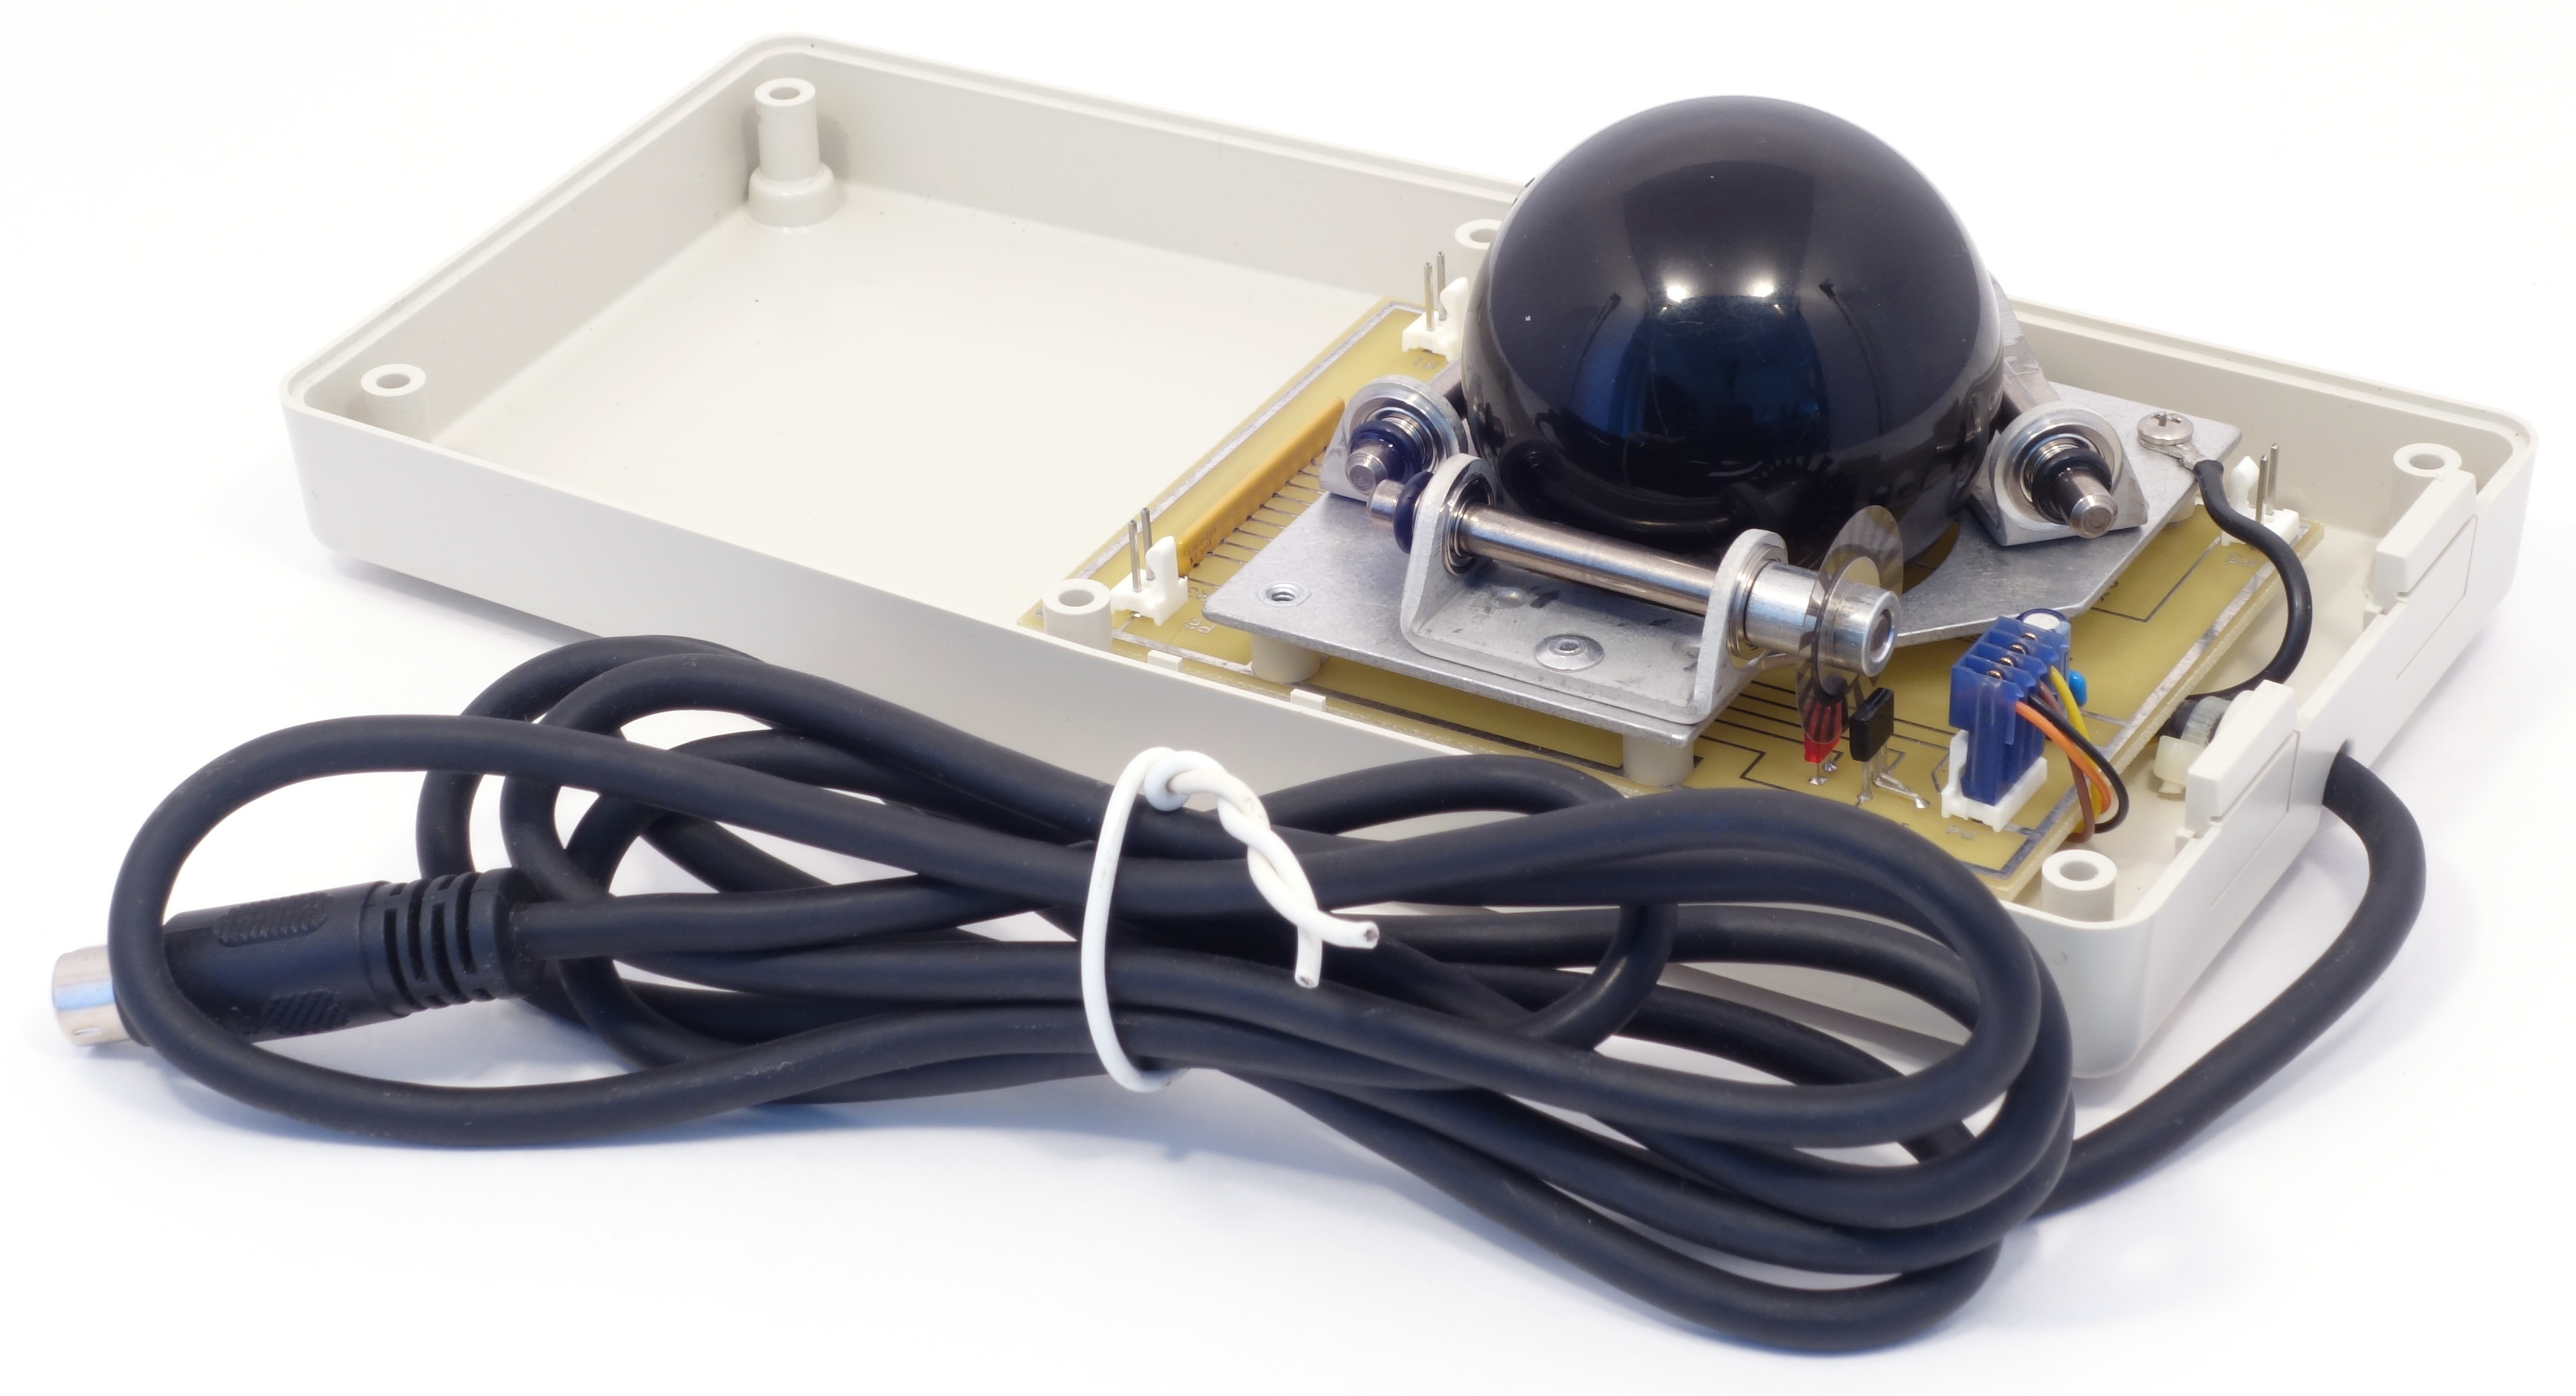
\includegraphics[scale=0.4]{1993_evergreen_diamond_xl_trackball/inside_30.jpg}
    \caption{Diamond XL trackball disassembled}
    \label{fig:DiamondXLInside}
\end{figure}

\begin{thebibliography}{9}
\bibitem{evergreen} Evergreen Systems International home page. \url{https://web.archive.org/web/19970102174426/http://trackballs.com:80/}
\bibitem{dtxl3} Keyton Computer -- Trackball \url{http://keyton.co.jp/products/UEVE/DTXL3.html}
\bibitem{hphil} Diamond XL HP-HIL trackball \url{https://web.archive.org/web/19970328230321/http://www.trackballs.com/xlhil.htm}
\bibitem{nasa} NASA Tech Briefs, November 1993. Volume 17, No. 11. -- p. 60 \url{https://archive.org/details/NASA_NTRS_Archive_20100030364/page/n59/mode/2up}
\end{thebibliography}
\end{document}
